% !TeX spellcheck = de_DE
\section{Organisation}
\subsection{Grundelemente der Organisationsgestaltung}
\begin{multicols}{2}
	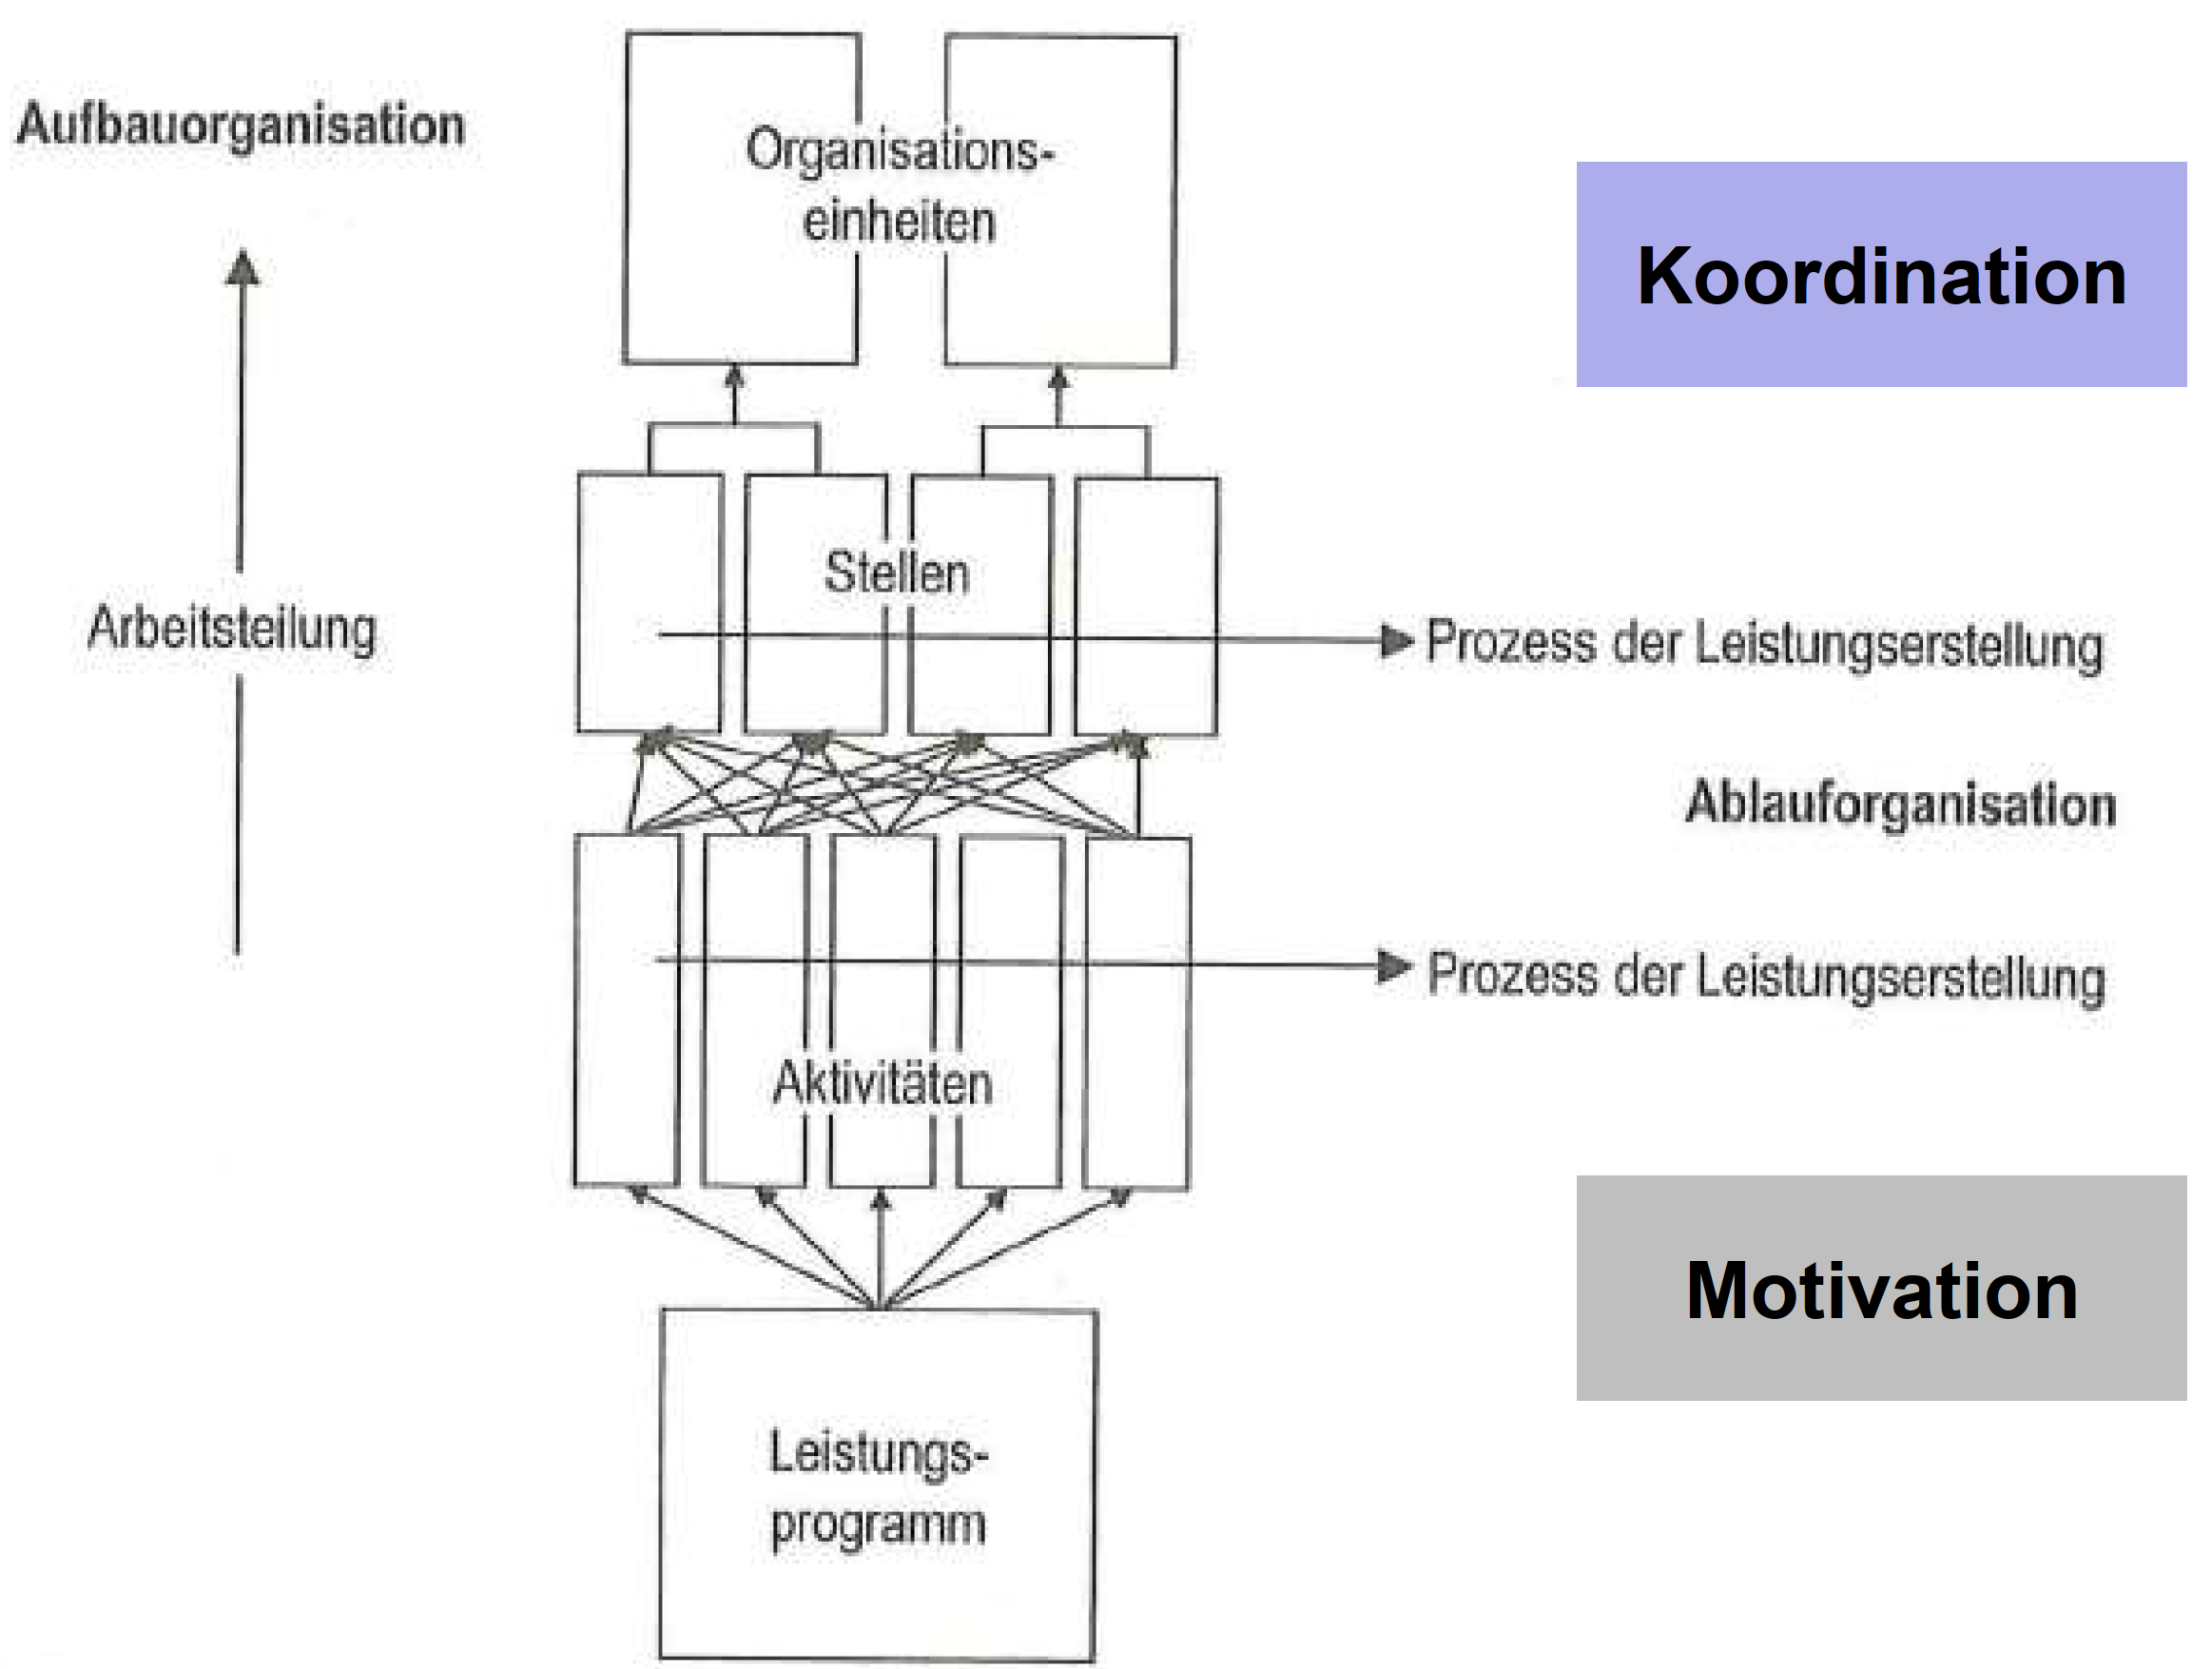
\includegraphics[width=1\linewidth]{images/grundelemente_1}
	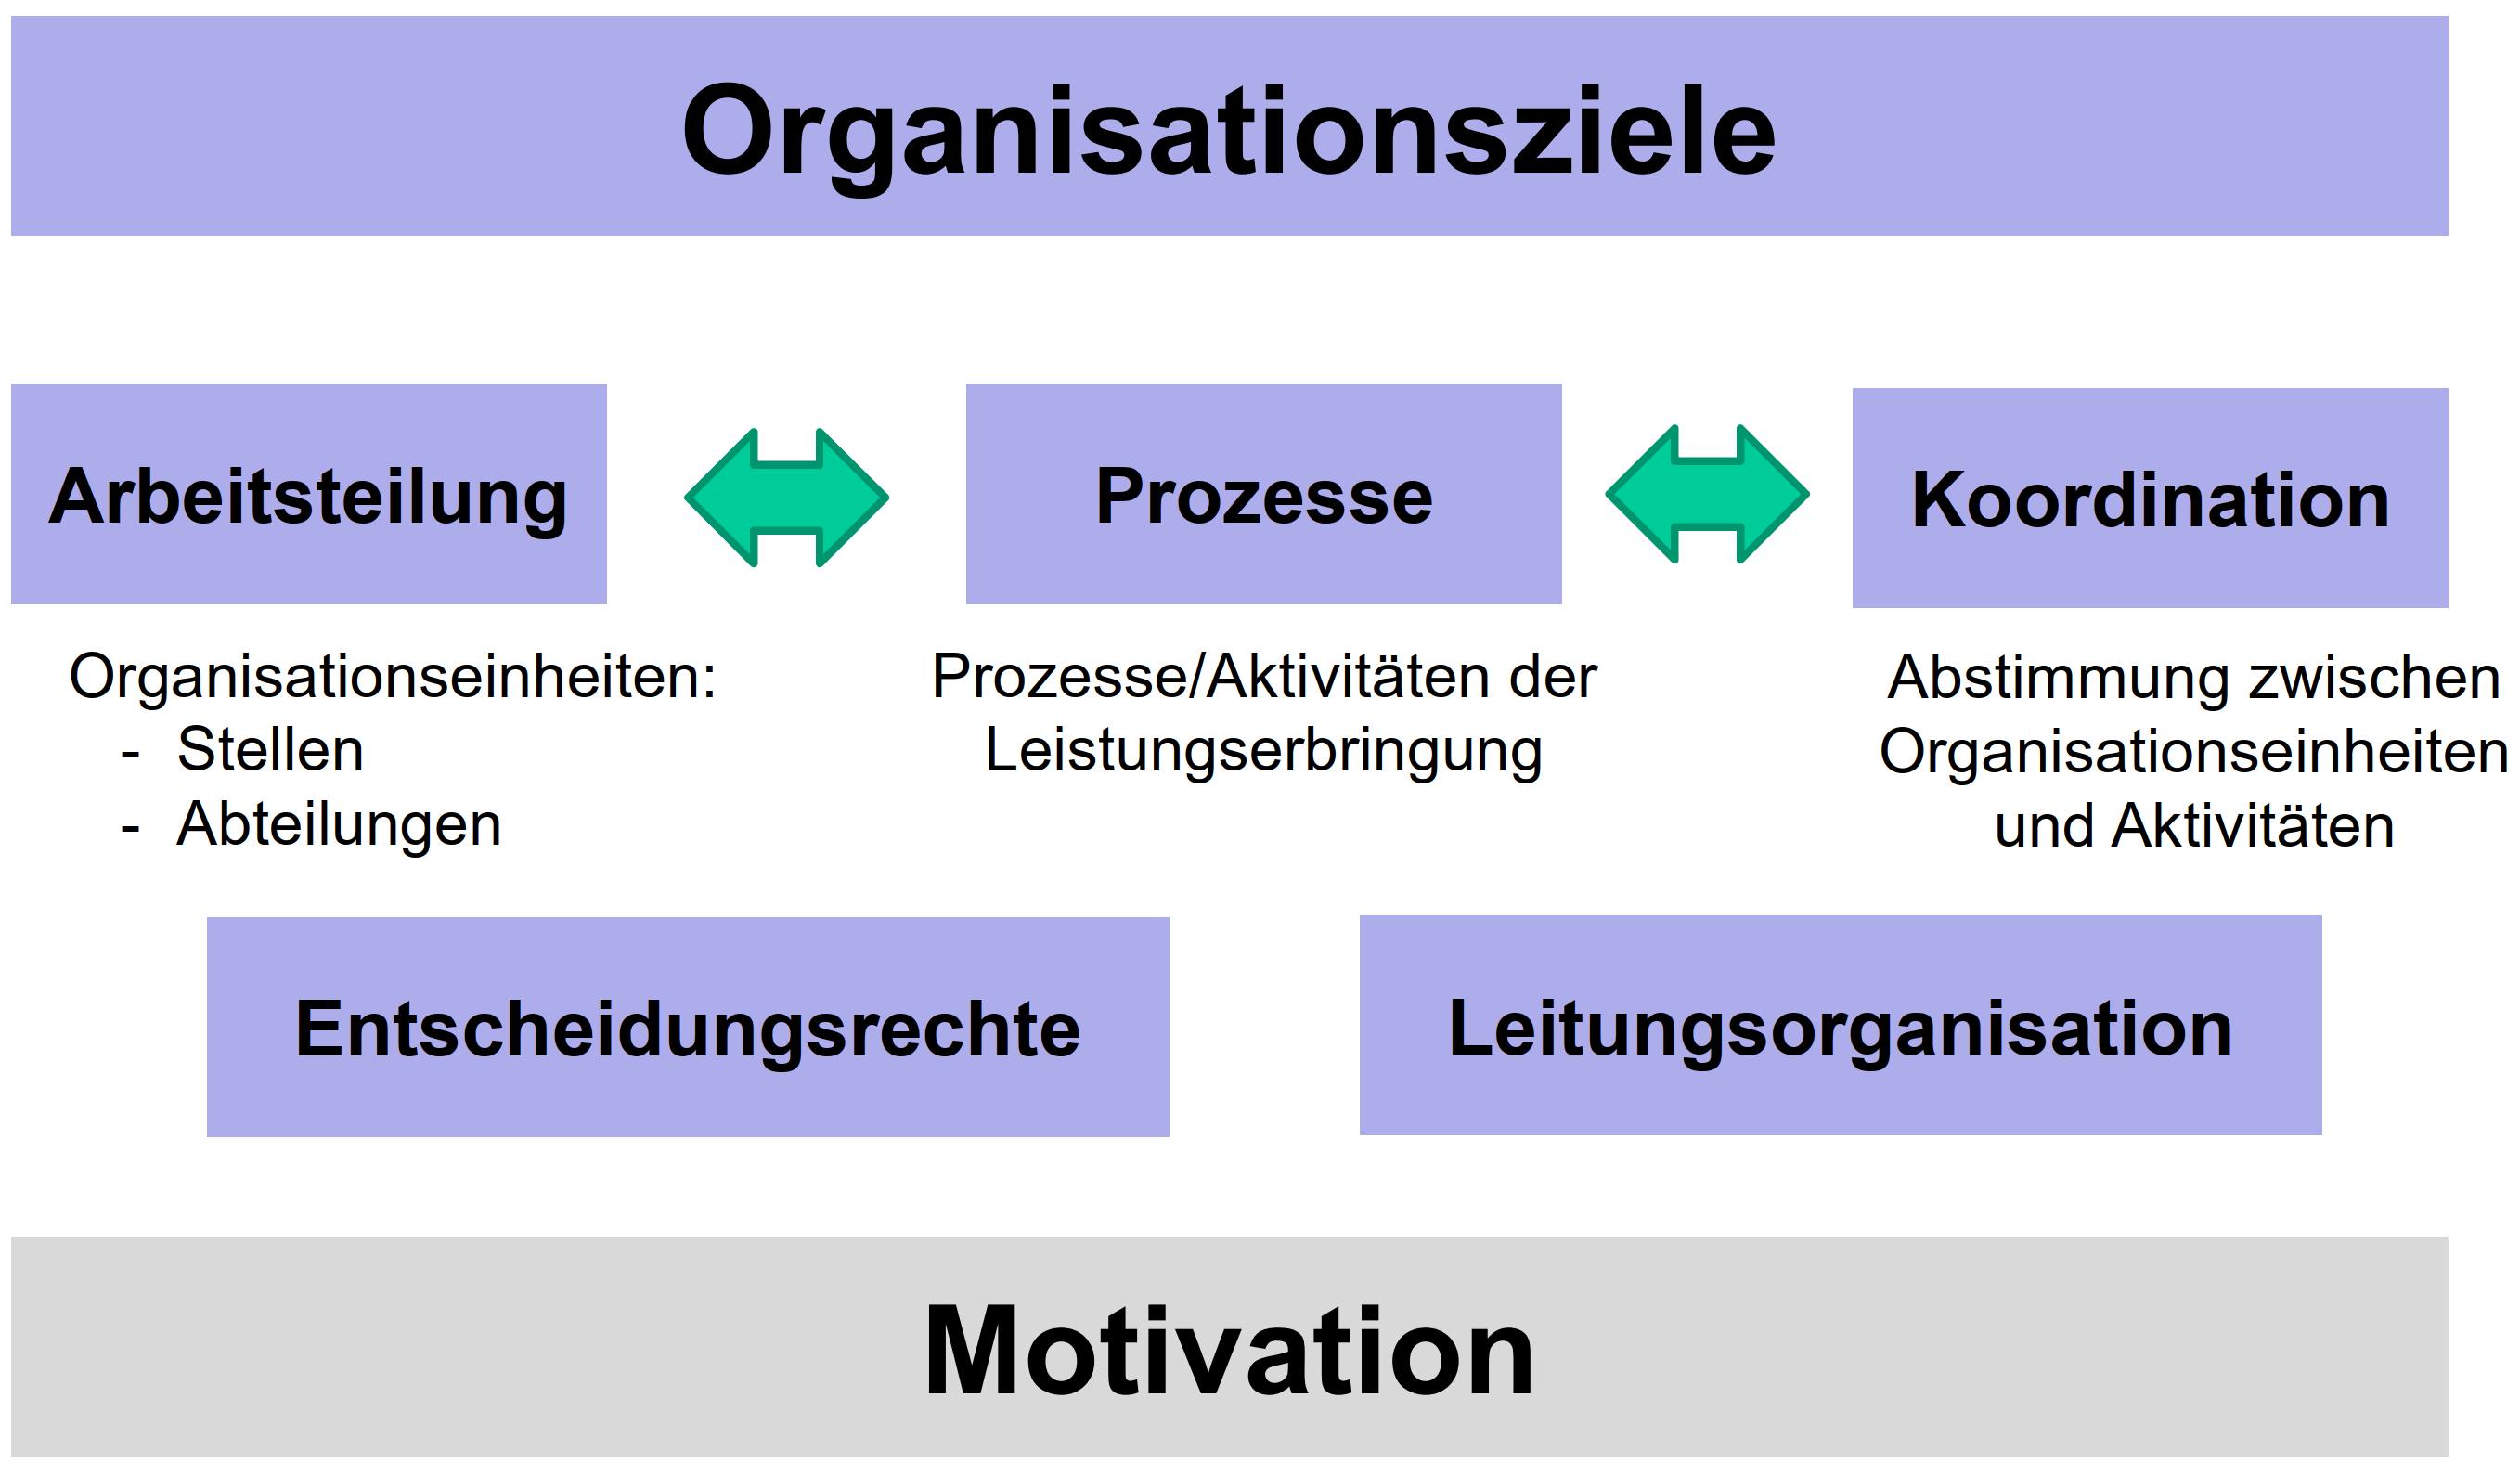
\includegraphics[width=1\linewidth]{images/grundelemente_2}
\end{multicols}

\subsubsection{Organisationsziele}
\begin{itemize}
	\item Ableitung von Organisationszielen
	\begin{enumerate}
		\item Sachziel: Welche Leistungen wollen wir erbringen (Leistungsprogramm)?
		\item Formalziel: Betriebswirtschaftliche Ziele zur Rentabilität und Wachstum einer Organisation.
	\end{enumerate}
	\item  Mögliche Zielsetzungen für Organisationsgestaltung
	\begin{enumerate}
		\item Effizienz/Effektivität der Leistungserbringung der Organisation in der aktuellen Situation (Exploitation): z.B.:
		\begin{itemize}
			\item Gewinn, Marktanteile, Umsatz
			\item Margen: Eigenkapital-/Umsatzrendite
		\end{itemize}
		\item Grössere Veränderungen für die Organisation ( Exploration )
		\begin{itemize}
			\item Neue Geschäftsmodelle
			\item Disruptive Produkte/Innovationen/Technologien
			\item Neue Märkte erschliessen
		\end{itemize}
	\end{enumerate}
\end{itemize}

\subsubsection{Arbeitsteilung}
\begin{itemize}
	\item Mengenteilung
	\begin{itemize}
		\item Verschiedene Akteure führen gleichartige Aktivitäten an gleichartigen	Objekten bzw. Subjekten durch
		\item Beispiel: Sachbearbeiter teilen Kunden nach Anfangsbuchstaben	des Nachnamens auf
		\item Vornehmlich zur einfachen Ausweitung von Kapazitäten
		\item Keine Spezialisierungsvorteile
	\end{itemize}
	\item  Artenteilung (Spezialisierung)
	\begin{itemize}
		\item Unterschiedliche Akteure / Abteilungen spezialisieren sich auf bestimmte Aktivitäten
		\item Spezialisierungseffekte z.B. Lernkurveneffekte
		\item Effektivität und Effizienz sind steigerbar z.B. günstigere Arbeitskräfte, höhere Leistungsfähigkeit, kürzere Einarbeitungszeiten
	\end{itemize}
	\item  Artenteilung (verrichtungsorientiert)
	\begin{itemize}
		\item Akteure spezialisieren sich nach Verrichtungen bzw. auf bestimmte	Aktivitäten
		\item Funktionale Organisation
	\end{itemize}
	\item  Artenteilung (objektorientiert)
	\begin{itemize}
		\item Akteure spezialisieren sich auf Objekte bzw. Subjekte mit / an denen sie Aktivitäten ausführen
		\item Divisionale Organisation (Sparten- oder Geschäftsbereichsorganisation)
	\end{itemize}
\end{itemize}

\subsubsection{Stellen}
Eine Stelle bildet die kleinste aufbauorganisatorische Einheit. Sie entsteht durch die dauerhafte Zuordnung von Aufgaben auf eine oder mehrere Personen. 

\paragraph{Merkmale}
\begin{enumerate}
	\item Dauerhafte Stellenaufgabe
	\item Stelleninhaber
	\item Kompetenzen
	\item Verantwortung
\end{enumerate}

\paragraph{Kompetenzen}
Kompetenzen sind die einem Stelleninhaber übertragenen formalen Rechte und Befugnisse. Sie legitimieren ihn zu den
Handlungen, die zur ordnungsgemässen Erfüllung der Stellenaufgabe notwendig sind.
\begin{itemize}
	\item Durchführungskompetenzen
	\begin{itemize}
		\item Ausführung: Arbeitsrhythmus und -methode
		\item Verfügung: Objekte, Sachmittel und Information anfordern
		\item Antrag: Bei anderer Stelle beantragen
		\item Entscheidung: Verbindliche Entscheide für eigene Stelle fällen
	\end{itemize}
	\item Leitungskompetenzen
	\begin{itemize}
		\item Entscheidung: Verbindliche Entscheide für fremde Stellen fällen
		\item Weisung: Anderen Stellen Aktivitäten zuweisen
		\item Richtlinien: Allgemeine Regelungen vorgeben
		\item Kontrolle: Ergebnisse oder Verfahren kontrollieren
	\end{itemize}
\end{itemize}

\subsubsection{Abteilungen}
Eine Abteilung ist eine unbefristete Zusammenfassung von Organisationseinheiten unter einer gemeinsamen Leitungsstelle.
\begin{multicols}{2}
	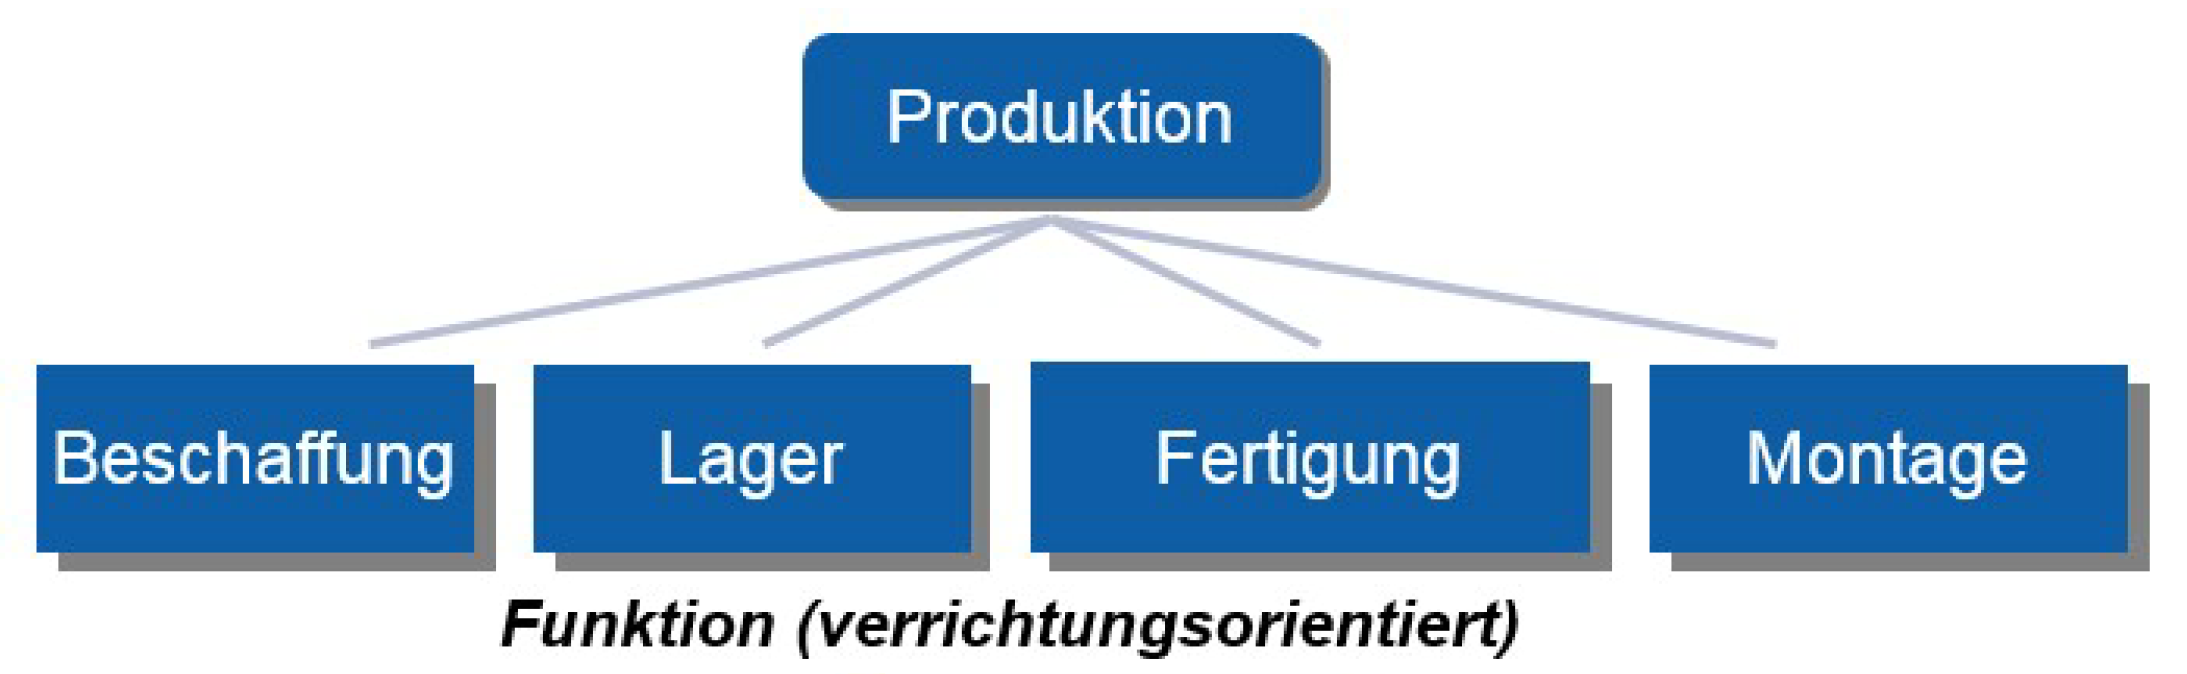
\includegraphics[width=1\linewidth]{images/abteilung_1}
	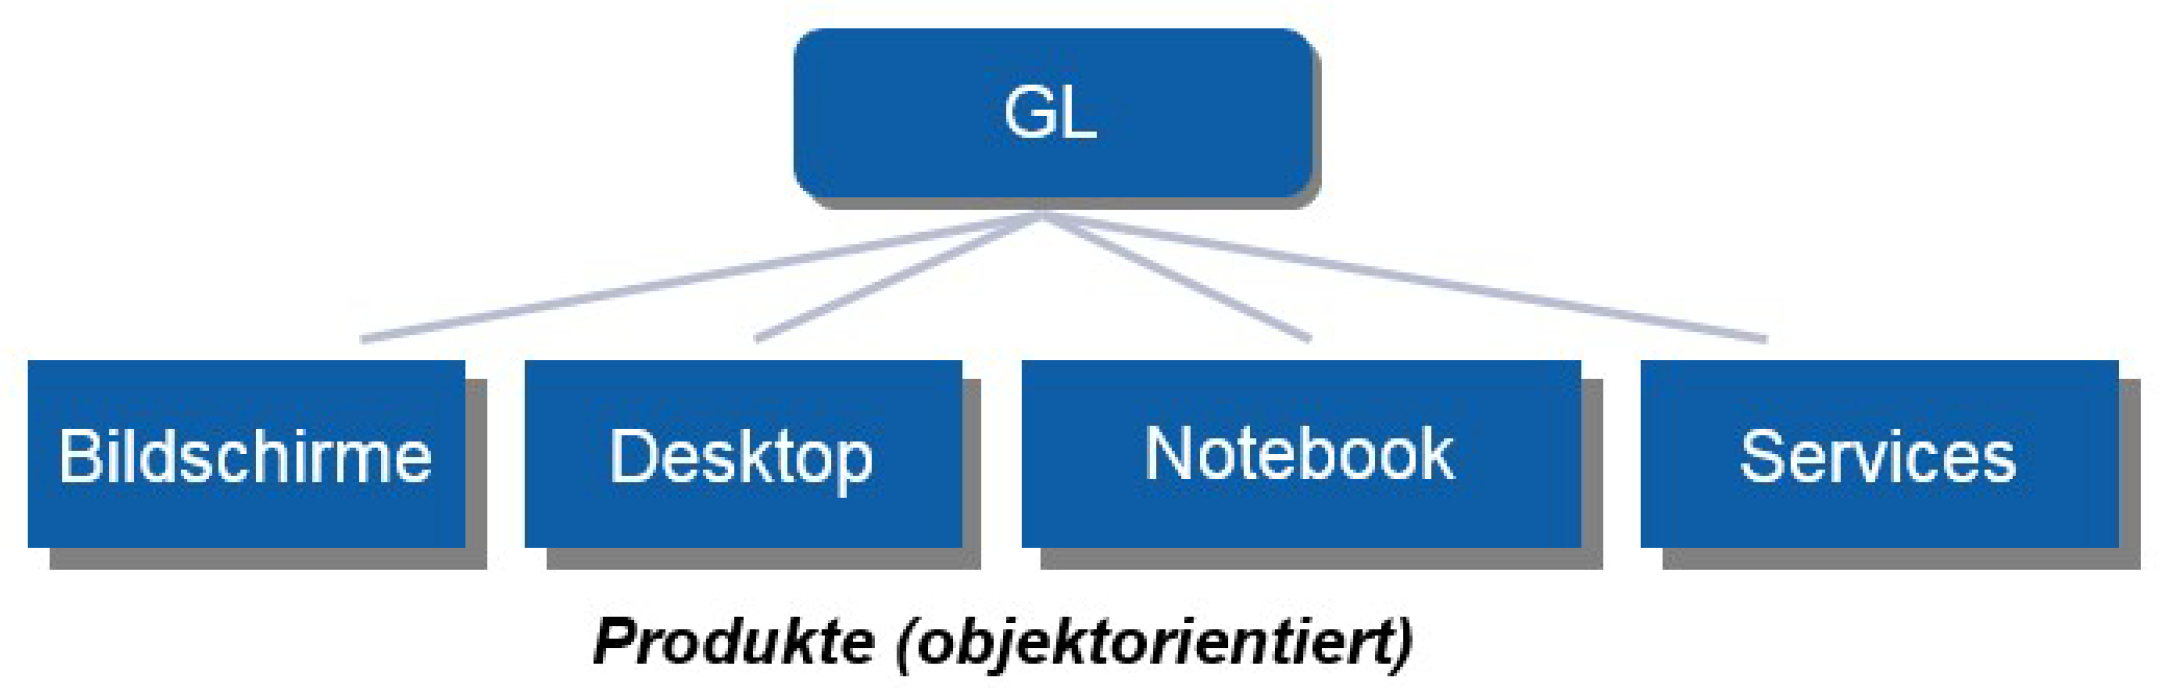
\includegraphics[width=1\linewidth]{images/abteilung_2}
\end{multicols}

\subsubsection{Prozessorientierung / -management als Notwendigkeit}
Prozessmanagement sind alle planerischen, organisatorischen und kontrollierenden Massnahmen zur zielgerichteten Steuerung der Wertschöpfungskette eines Unternehmens in Hinblick auf die Zielsetzung Kosten, Zeit, Qualität, Innovationsfähigkeit und Kundenzufriedenheit. \\
Dessen Anwendung unterstützt die
\begin{itemize}
	\item Reduktion von gegenseitigen Abhängigkeiten in Aktivitäten
	\item Verringerung der Schnittstellenproblematik
	\item ganzheitliche Prozessverantwortung (Selbstabstimmung, Motivation)
	\item bessere (interne und externe) Kundenorientierung
	\item Konzentration auf wertschöpfende Aktivitäten
	\item kontinuierliche Verbesserungsprozesse
\end{itemize}

\subsubsection{Koordinationsbedarf}
Koordination beinhaltet die Abstimmung von Einzelaktivitäten in Hinblick auf ein übergeordnetes Gesamtziel.
\begin{itemize}
	\item Begründung
	\begin{itemize}
		\item Art und Ausmass der Arbeitsteilung bestimmen Spezialisierungsvorteile, begründen aber auch Koordinationsbedarf.
		\item Koordinationsbedarf ergibt ich immer dann, wenn zwischen verschiedenen Tätigkeits- und Entscheidungsbereichen
		Schnittstellen (Berührungspunkte) und Interdependenzen bestehen.
		\item Koordinationsbedarf besteht auf allen Ebenen der Arbeitsteilung: zwischen Stellen, Teams, Abteilungen, ...
	\end{itemize}
	\item Arten von Interdependenzen
	\begin{enumerate}
		\item (sequentielle vs. reziproke) Prozessinterdependenzen
		\item Ressourceninterdependenzen
		\item Marktinterdependenzen
	\end{enumerate}
	\item bei Mengenteilung
	\begin{itemize}
		\item Relativ geringe Interdependenzen zwischen einzelnen Aktivitäten und Prozessen zwischen Organisationseinheiten.
		\item Vornehmlich Nutzung gemeinsamer Ressourcen («Skaleneffekte») und Bemühungen zur Vereinheitlichung der Leistungserbringung
	\end{itemize}
	\item bei verrichtungsorientierter Artenteilung
	\begin{itemize}
		\item Prozesse der Leistungserbringung und arbeitsteilig erbrachte Leistungsergebnisse (Output) müssen intensiv aufeinander abgestimmt werden: Mengen, Qualitäten, Termine.
		\item Output von Organisationseinheiten sind Inputs anderer Einheiten (Prozessinterdependenzen).
	\end{itemize}
	\item bei objektorientierter Artenteilung
	\begin{itemize}
		\item Höhere Unabhängigkeit zwischen jeweils bearbeiteten Objekten bzw. Subjekten.
		\item Zugriff auf zentrale Services im Unternehmen (Personal, Forschung \& Entwicklung)
	\end{itemize}
\end{itemize}

\subsubsection{Bedarfsdeckung}
\paragraph{Persönliche Koordinationsmechanismen}
Kommunikation zwischen den für die abzustimmenden Aktivitäten verantwortlichen Akteuren.
\begin{itemize}
	\item Persönliche Weisung
	\begin{itemize}
		\item Koordination vertikal über Hierarchieebenen hinweg
		\item Beispiel: Steuerung und Kontrolle durch Vorgesetzten
	\end{itemize}
	\item Selbstabstimmung
	\begin{enumerate}
		\item Koordination horizontal auf gleicher Hierarchieebene
		\item Z.B. Meetings zum Informationsaustausch, Ausschüsse
	\end{enumerate}
	\item Organisationskultur
	\begin{itemize}
		\item Informelle Koordination
		\item verankerte Normen, Werte und Verhaltensmuster ermöglichen, das sich stabile Verhaltenserwartungen bilden
		\item An diesen können sich Akteure aus unterschiedlichen organisationalen Einheiten orientieren
	\end{itemize}
\end{itemize}

\paragraph{Technokratische Koordinationsmechanismen}
Personenunabhängige Koordination über formale Vorgaben.
\begin{itemize}
	\item Anreizsysteme
	\begin{itemize}
		\item Effekte auf individuelle Ziele (Vorteile, Sanktionen) werden an Entscheidungen und Handlungen in der Organisation gekoppelt
		\item Ausrichtung auf effektive und effiziente Leistungserbringung
		\item Beispiele: Profit Center, interne Verrechnungspreise (Organisational); Karrierewege, Entlohnungssysteme (Personal)
	\end{itemize}
	\item Planung
	\begin{enumerate}
		\item Periodische Vorgaben zu Inputs, Prozessen und Outcomes (Mengen, Qualitäten, Termine), die für mehrere Organisationseinheiten gelten
		\item Output-orientierte Steuerung
	\end{enumerate}
	\item Verfahrensvorgaben
	\begin{itemize}
		\item Definition genereller Regelungen für Leistungserstellung und -verwendung
		\item Input-orientierte Steuerung
	\end{itemize}
\end{itemize}

\subsubsection{Verteilung von Entscheidungsrechten}
\begin{itemize}
	\item \textbf{Zentralisierte vs. dezentralisierte Organisation:} Verteilung von Entscheidungsrechten auf oberste Unternehmensleitung (zentralisiert) vs. Es werden umfangreich Entscheidungsbefugnisse an tiefere Hierarchieebenen «delegiert».
	\item \textbf{Delegation:} Delegation beinhaltet die dauerhafte Übertragung von Entscheidungsaufgaben sowie zugehöriger Kompetenzen und	Verantwortung an hierarchisch nachgeordnete Stellen.
	\item \textbf{Subsidiaritätsprinzip:} Entscheidungen und Aktivitäten sollten immer an der untersten Ebene angesiedelt werden, die zur adäquaten Ausführung gerade noch in der Lage ist.	
\end{itemize}

\paragraph{Delegation}
Delegation ist tendenziell dann eher umzusetzen
\begin{itemize}
	\item je kürzer die zeitliche Reichweite der Entscheidungen
	\item je geringer die Auswirkungen einer Entscheidung auf andere Bereiche bzw. auf das ganze Unternehmen sind
	\item je stärker es um rein sachtechnische Entscheidungen geht (im Gegensatz zu Entscheidungen, die direkte Auswirkungen auf Mitarbeiter haben)
	\item je geringer das Risiko und je sicherer die Entscheidungssituation ist
	\item je stärker es sich um Routinefälle handelt
\end{itemize}

\paragraph{Leitungsorganisation}
\begin{itemize}
	\item Regelt, entlang welcher hierarchischer Leitungsbeziehungen steuernd und koordinierend eingegriffen werden darf
	\item D.h., welche Stellen und Organisationseinheiten welchen anderen weisungsbefugt sind (Verteilung von Weisungsrechten)
	\item Organisation bzw. Struktur der Leitungsbeziehungen (Konfiguration von Über- und Unterordnungsbeziehungen)
\end{itemize}
Konfiguration ist die äussere Form des Stellengefüges einer Organisation.

\paragraph{Gestaltungsentscheidungen}
\begin{itemize}
	\item Wie viele Akteure sollen einer übergeordneten Organisationseinheit unterstellt werden (Leitungsspanne)?
	\item Wie viele Hierarchieebenen soll ein Unternehmen aufweisen?
	\item Nach welchem System sollen die Weisungsbeziehungen geregelt werden (Einlinien- vs. Mehrliniensysteme)
\end{itemize}

\subsubsection{Leitungsspanne}
Die Leitungsspanne beinhaltet die Anzahl der einer Leitungsstelle unmittelbar unterstellten Personen.
\begin{itemize}
	\item Es gibt keine - für alle Organisationseinheiten einheitliche – optimale Leitungsspanne
	\item Entscheidend ist, wie viele Mitarbeiter ein Vorgesetzter steuern und koordinieren kann.
	\item Einflussfaktoren:
	\begin{enumerate}
		\item Aufgabenmerkmale (Beobachtbarkeit)
		\item Persönliche Merkmale
		\item Führungsstil des Vorgesetzten
		\item Informations- und kommunikationstechnische Sachmittel (IKT)
		\item Organisatorische und personelle Massnahmen (Umstrukturierung)
	\end{enumerate}
\end{itemize}

\paragraph{Hierarchieebenen}
Die Leitungstiefe ist die Zahl der hierarchischen Leitungsebenen in einem Unternehmen.
\begin{itemize}
	\item Anzahl Hierarchieebenen hängt eng zusammen mit der Gestaltung der Leitungsspannen (ceteris paribus)
	\item Anzahl Hierarchieebenen kann in Unternehmen zwischen Bereichen variieren – notwendige Anpassung an stark divergierende Rahmenbedingungen
\end{itemize}
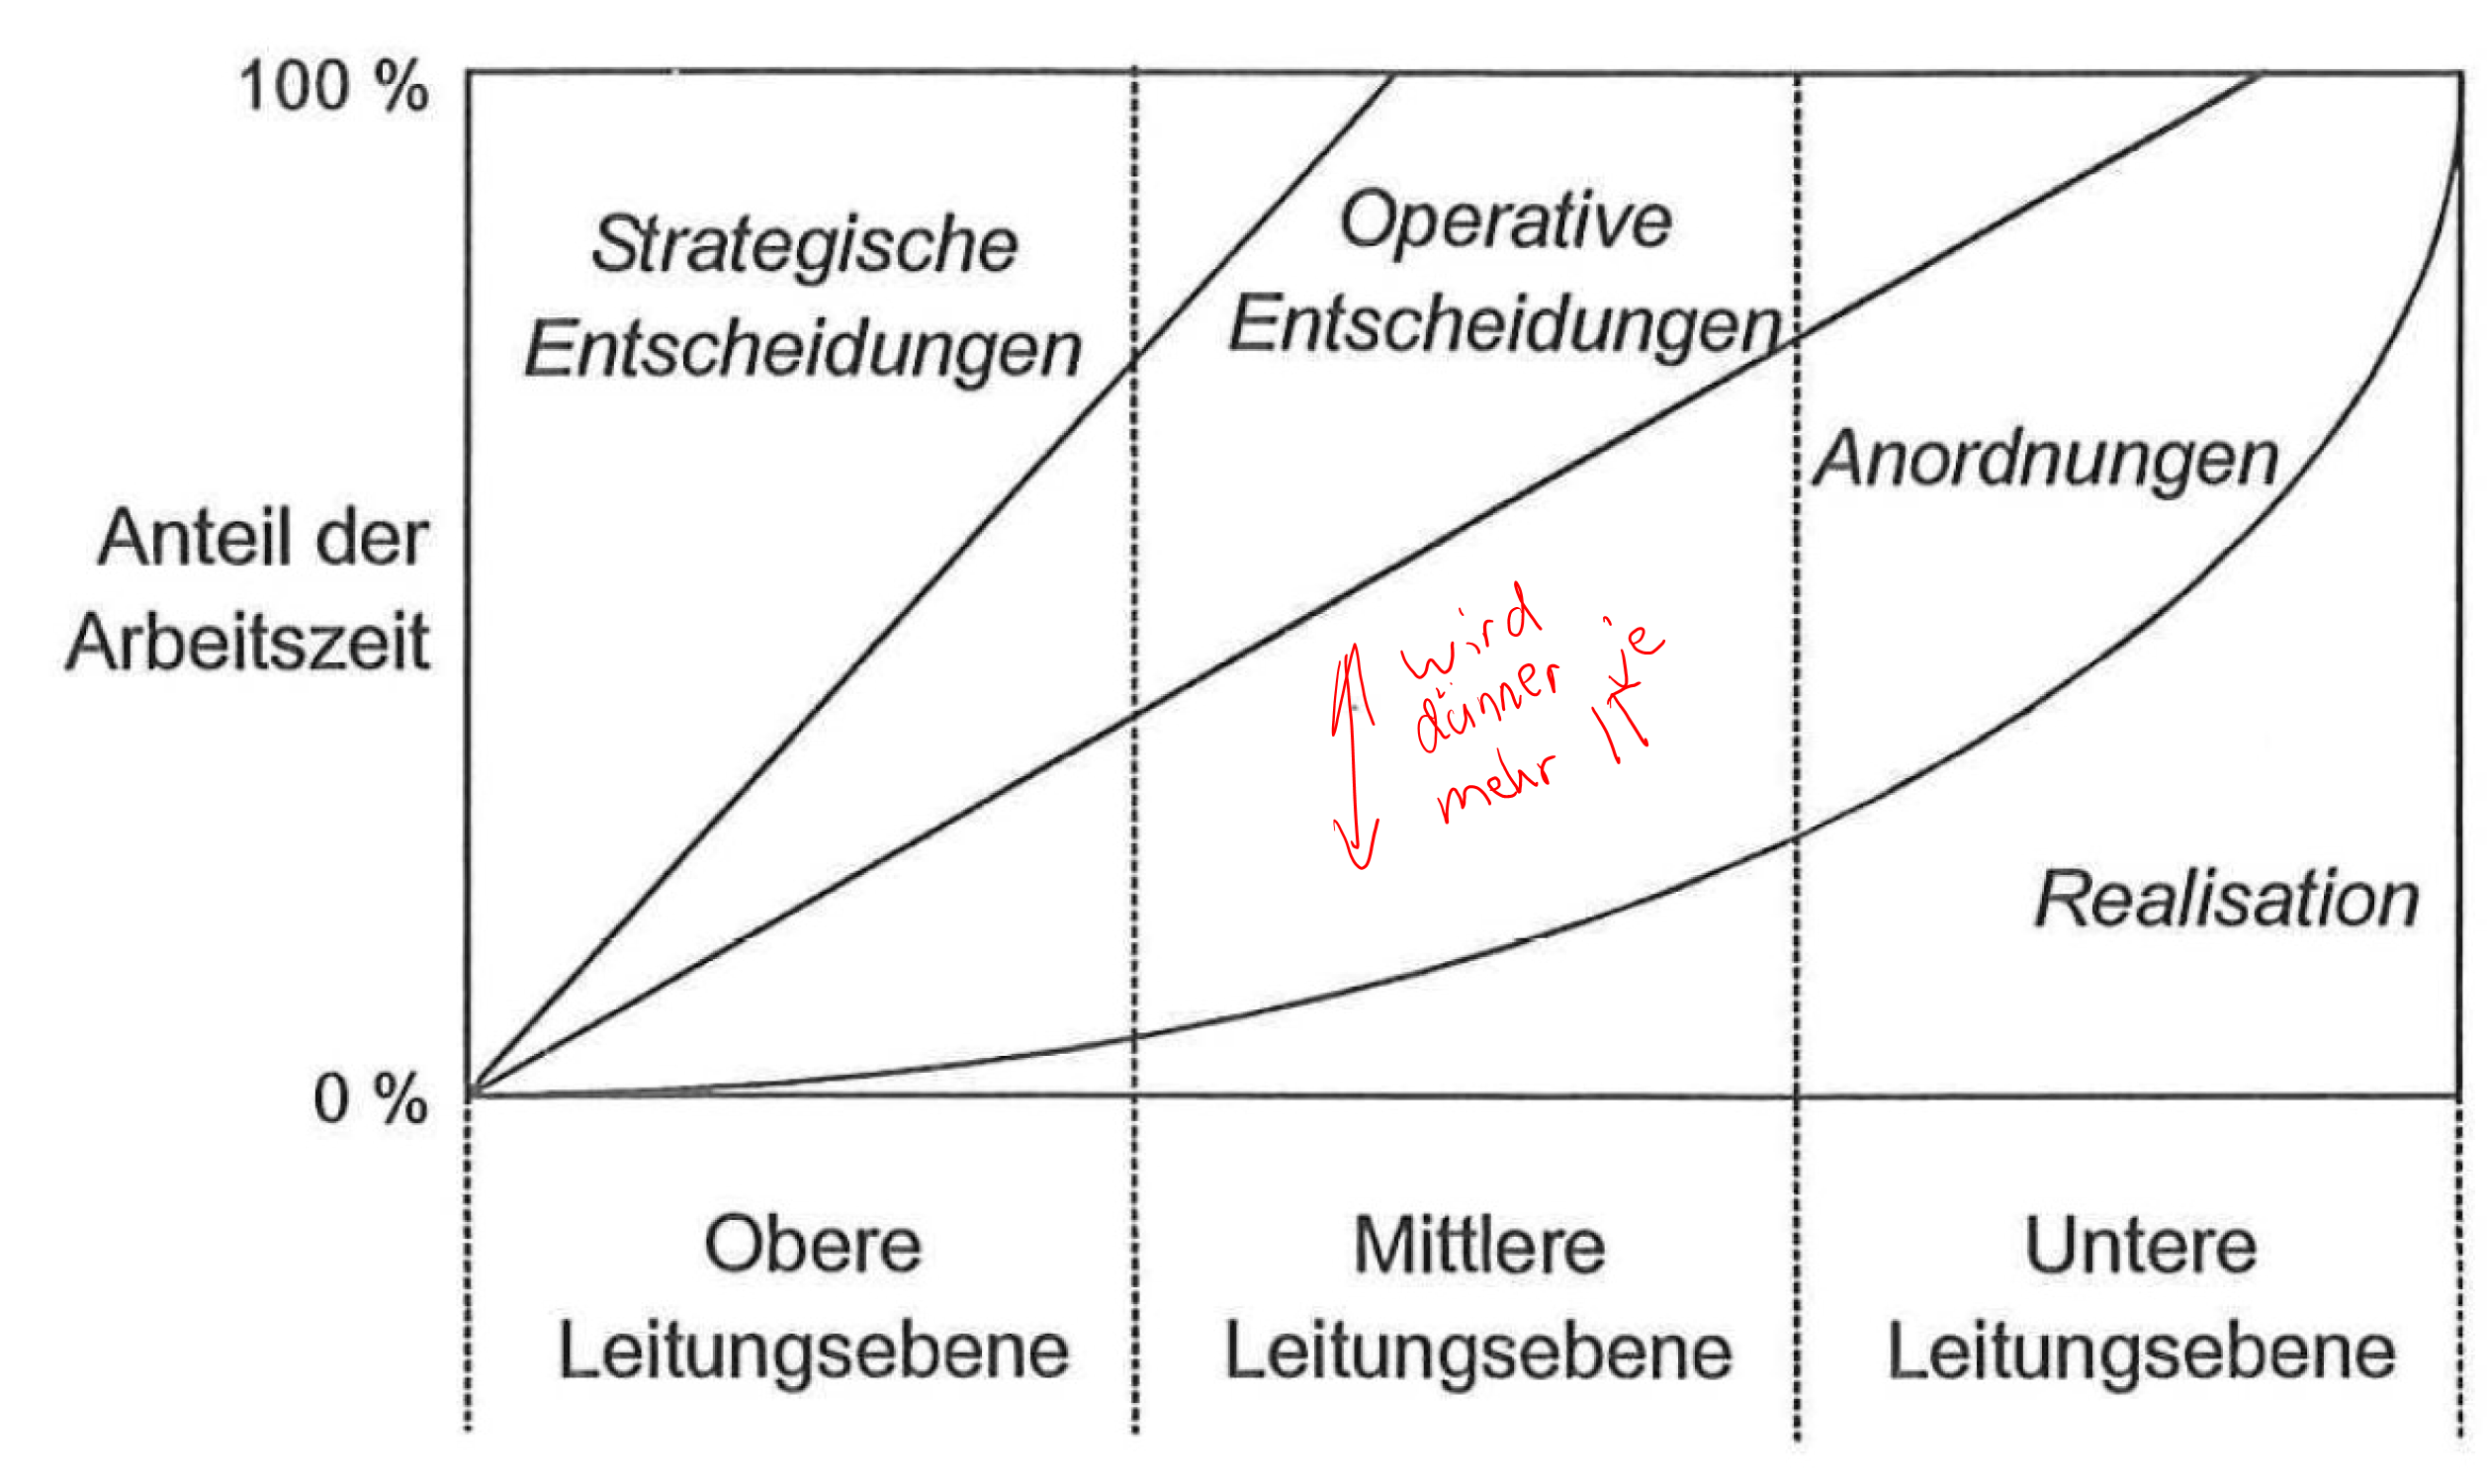
\includegraphics[width=0.4\linewidth]{images/leitungsebenen}

\subsubsection{Weisungsbeziehungen}
\begin{multicols}{2}
	\paragraph{Einliniensysteme}
	In einem Einliniensystem erhält jede untergeordnete Stelle nur von einer übergeordneten Stelle Anweisungen.
	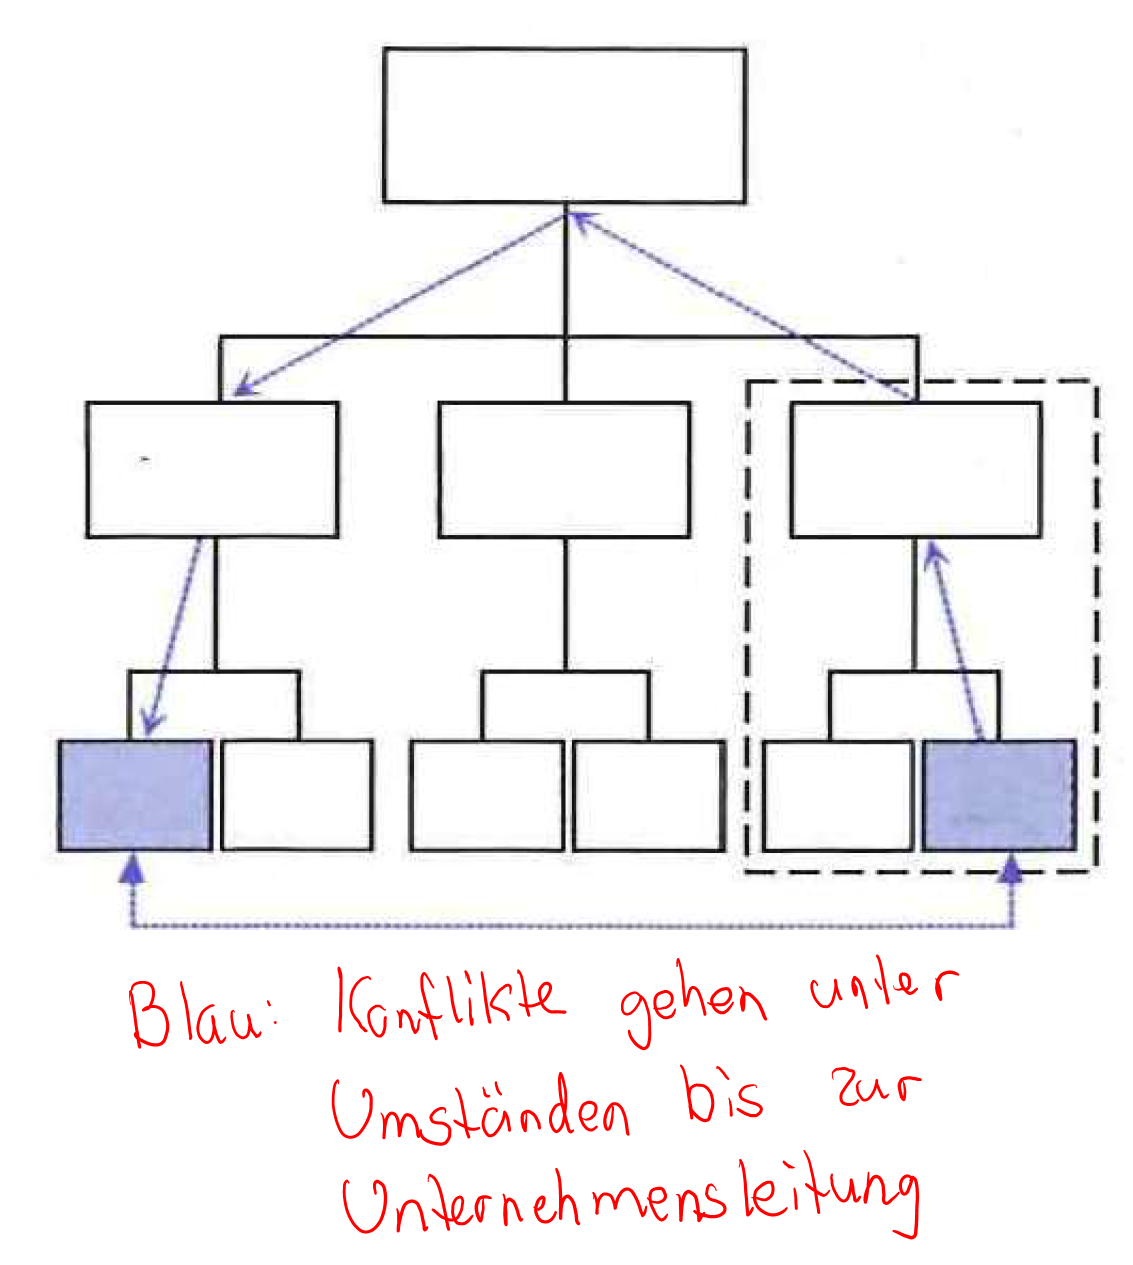
\includegraphics[width=0.7\linewidth]{images/einliniensystem} \\
	Vorteile:
	\begin{itemize}
		\item Eindeutige Regelung der Unterstellungsverhältnisse
		\item Klare Zuordnung von Aufgaben. Verantwortung und Kompetenzen; dadurch geringes Risiko von Konflikten
		\item Überschaubares und einfaches Leitungssystem (Einheit der Leitung und der Auftragserteilung)
		\item Lückenloser Informationsfluss top-down und bottom-up über alle Hierarchieebenen
		\item Gute Kontrollmöglichkeiten
	\end{itemize}
	
	\paragraph{Mehrliniensysteme}
	In einem Mehrliniensystem erhält eine untergeordnete Stelle von	mehreren übergeordneten Stellen Anweisungen.
	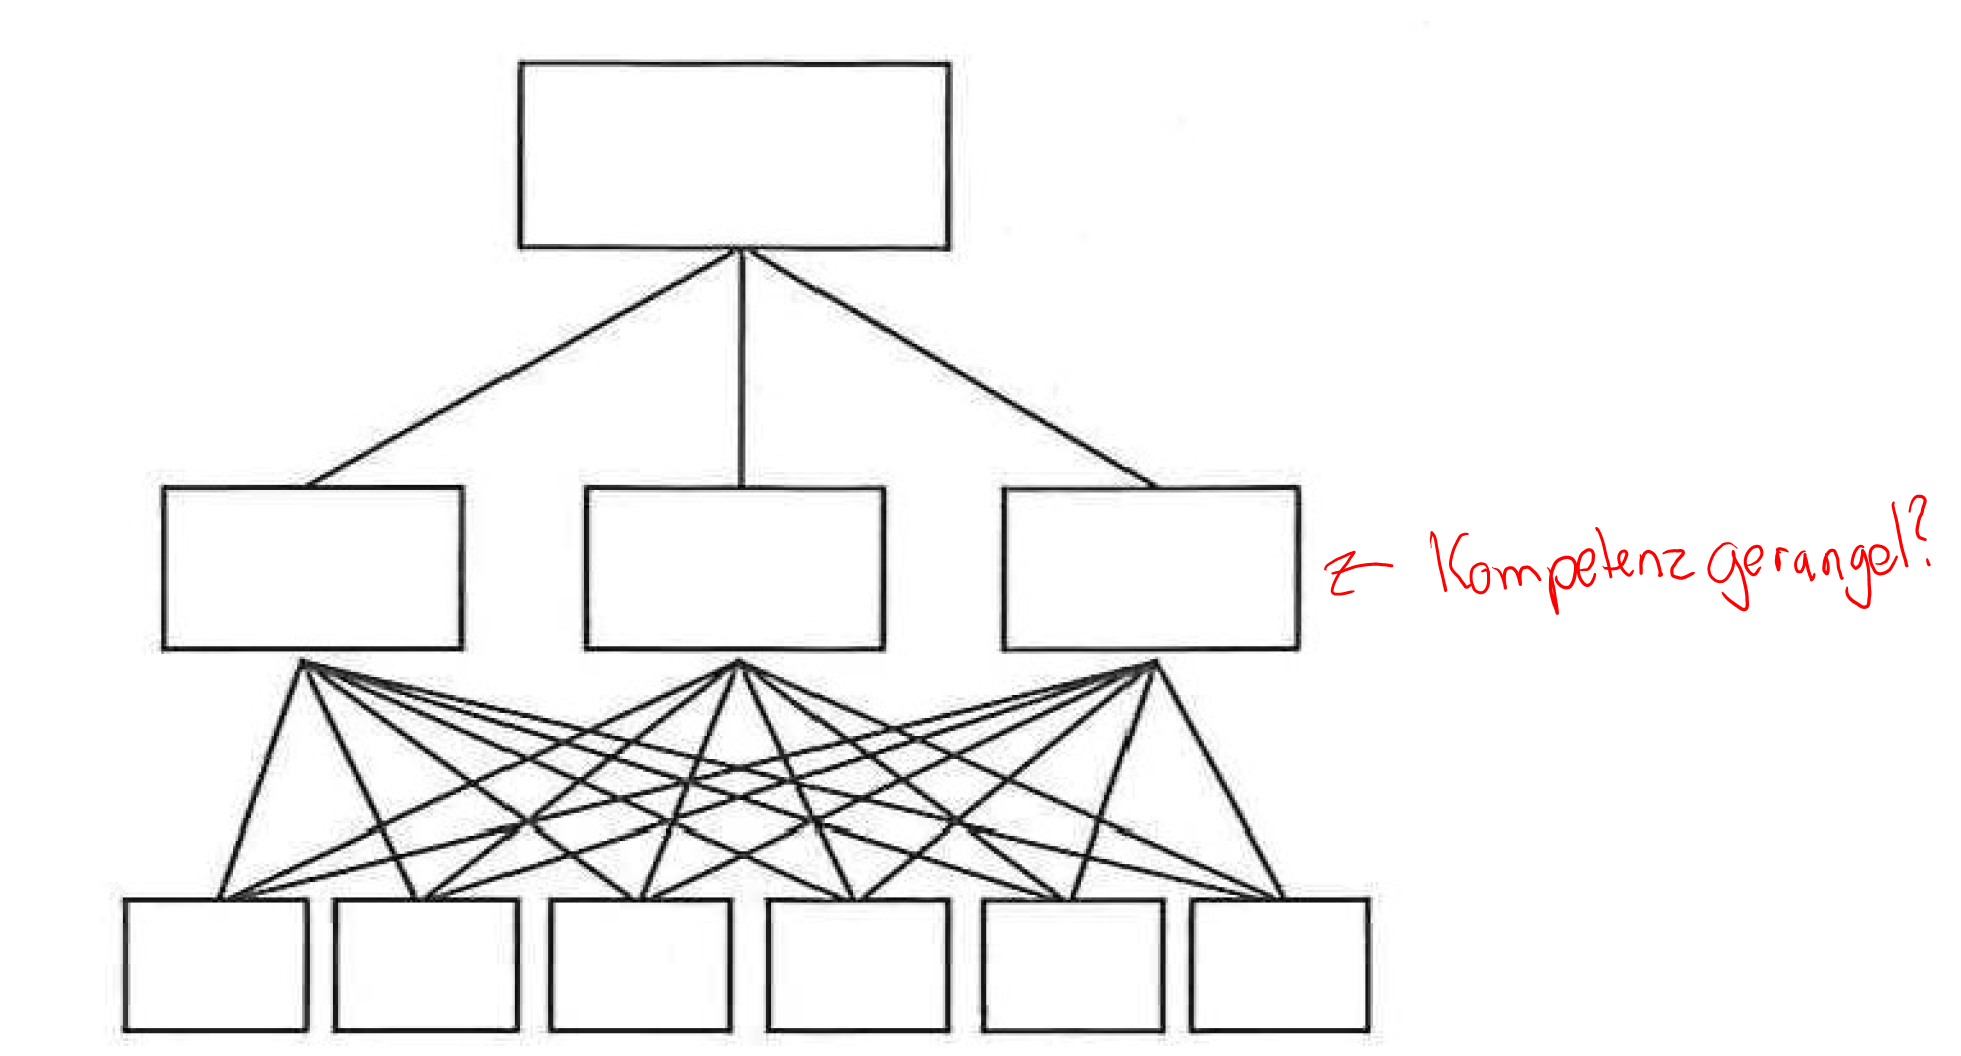
\includegraphics[width=1\linewidth]{images/mehrliniensystem}
	Vorteile:
	\begin{itemize}
		\item Spezialisierung der Leitung durch Verteilung einzelner Funktionen auf mehrere Instanzen
		\item Entlastung der Leitungsspitze
		\item Verkürzung der Informations- und Weisungswege
		\item Direkte und schnelle Kommunikation
		\item Betonung der fachlichen Autorität der Vorgesetzten; geringere hierarchische Distanz
		\item Mehrfachunterstellung fördert produktive Konflikte; dadurch hohe Problemlösungskapazität
	\end{itemize}
	\ \\ \ \\
\end{multicols}

\paragraph{Matrixsysteme}
In einem Matrixsystem erhält eine untergeordnete Stelle von zwei übergeordneten Stellen Anweisungen. \\
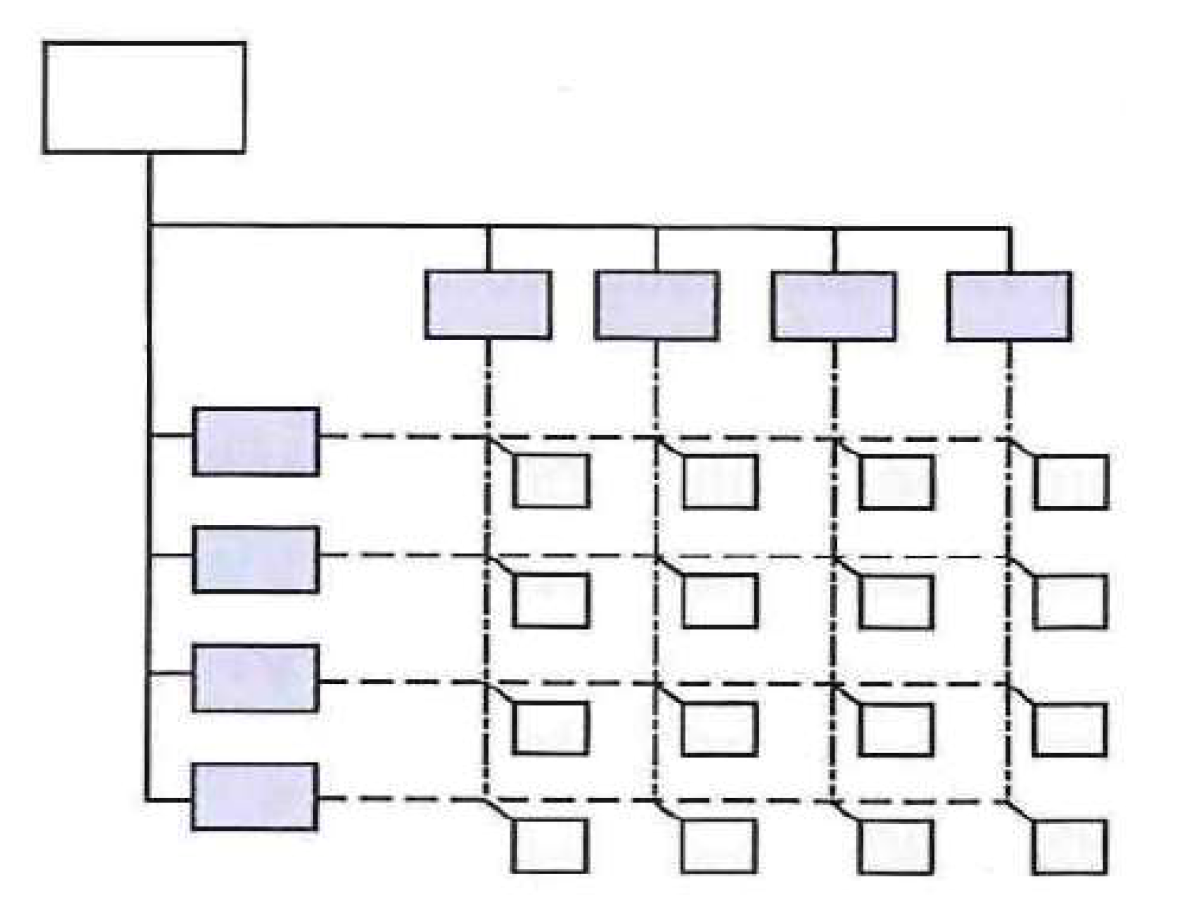
\includegraphics[width=0.35\linewidth]{images/matrixsystem}

\subsection{Einzelne Gestaltungsentscheidungen}
\subsubsection{Stellengestaltung}
\paragraph{Koordination}
Stellen bilden die kleinste organisatorischen Einheiten der Aufgabenerfüllung. Sie werden jeweils charakterisiert durch ein Bündel an Aktivitäten, deren Erfüllung dem Stelleninhaber dauerhaft zugewiesen wird.

\subparagraph{Koordinationsbezogene Gestaltungsregeln}
\begin{enumerate}
	\item Stelleninhaber sollen über Entscheidungs- und Weisungsrechte verfügen, die für die adäquate Aufgabenerfüllung notwendig sind.
	\item Es ist vorteilhaft, die mit einer Stelle verbundenen Rechte und Pflichten der Aufgabenerfüllung möglichst unabhängig von der konkreten Person eines Stelleninhabers zu formulieren (erleichtert Personalwechsel, macht unabhängiger von konkreten Personen)
	\item Rechte und Pflichten sollten derart gestaltet sein, dass sie von einer dafür qualifizierten Person unter normalen Umständen gut erfüllt werden können.
\end{enumerate}

\subparagraph{Abwägung}
Analog zu Abteilungsgliederung werden auch bei der Stellengestaltung Vor- und Nachteile einer starken Verrichtungsorientierung gegenübergestellt. Spezialisierungsvorteile ergeben sich bei funktionaler, verrichtungsorientierter Stellenbildung. Es ist allerdings stets zu hinterfragen, inwieweit die erzielbaren Spezialisierungsvorteile Nachteile bei (zusätzlichem) Koordinationsaufwand und die schlechtere Marktausrichtung aufwiegen!

\paragraph{Motivation}
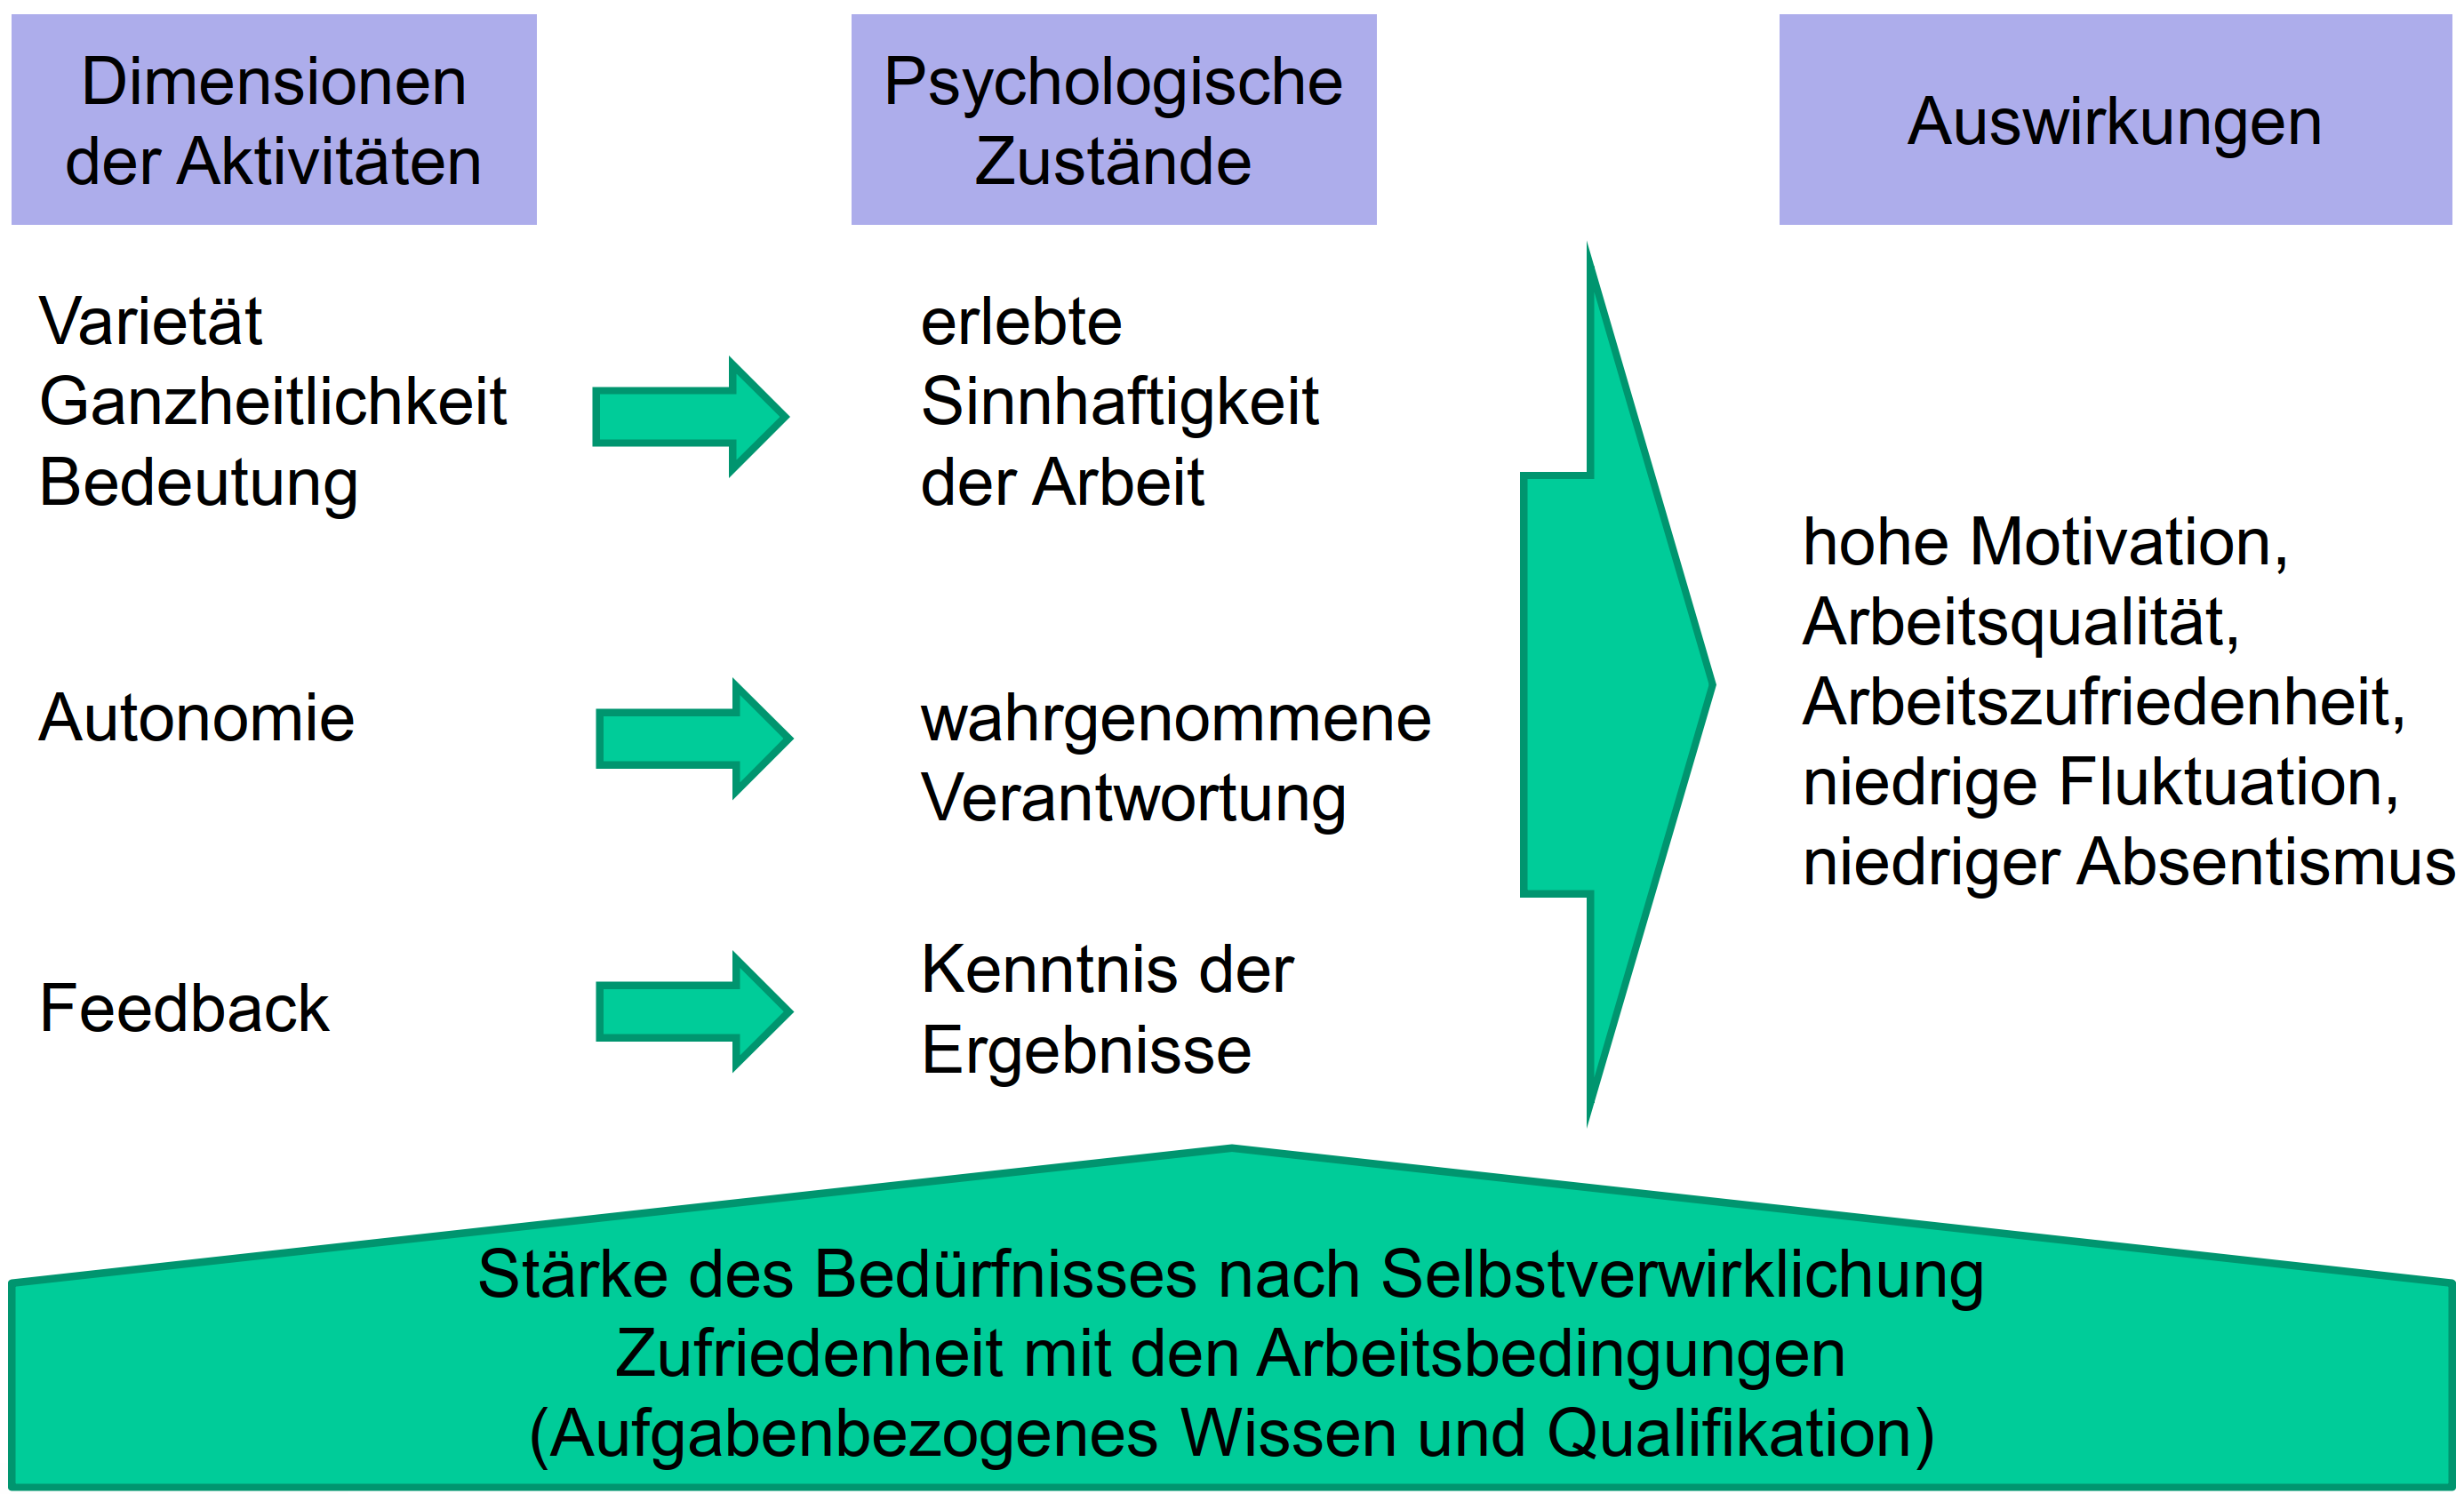
\includegraphics[width=0.5\linewidth]{images/motivation}

\subsubsection{Abteilungsbildung}
Abteilungsbildung ist immer dann notwendig, wenn die Zahl der Beschäftigten die Leitungskapazität eines einzelnen Vorgesetzten überschreitet z.B. wenn eine Organisation(seinheit) stark gewachsen ist oder die Aktivitäten komplexer oder variabler geworden sind. Zur Abteilungsbildung müssen Untereinheiten gebildet werden, deren jeweilige Leitungsperson Führungsaufgaben übernimmt. Der Begriff bezeichnet jede Form der Bildung von Untereinheiten unabhängig von Grösse und hierarchischem Rang der betroffenen Einheiten. \\
Zentrale Frage: Welche Stellen oder organisatorischen Einheiten sollen einer einheitlichen Verantwortung unterstellt werden?

\paragraph{Prinzip}
Grundsätzliches Prinzip: Fasse solche Stellen oder Organisationseinheiten zusammen, die möglichst viele Ähnlichkeiten und/oder Interdependenzen bezüglich derjenigen Aktivitäten aufweisen, die den relativ grössten Erfolgsbeitrag leisten! \\
Ähnlichkeit: z.B. in Bezug auf
\begin{itemize}
	\item verwendete Technologien
	\item realisierte Prozesse
	\item genutzte Ressourcen
	\item erforderliche Qualifikationen
	\item erstellte Produkte und Leistungen
	\item bediente Kunden und Märkte
\end{itemize}
Das Zusammenführen von ähnlichen Stellen oder Organisationseinheiten zu Abteilungen erlaubt Grössen- und Synergieeffekte!

\subparagraph{Interdependenzen}
Treten immer dort auf, wo Abhängigkeiten zwischen einzelnen Prozessen der Leistungserstellung bestehen.
\begin{itemize}
	\item Prozessinterdependenzen
	\item Ressourceninterdependenzen
	\item Marktinterdependenzen
\end{itemize}
Das Zusammenführen von Interdependenzen zwischen Stellen oder Organisationseinheiten zu Abteilungen ist aus organisationaler Sicht förderlich, weil die zur Leistungserbringung notwendigen Aktivitäten und die damit verbundenen Koordinationsmassnahmen innerhalb einer Abteilung leichter abgestimmt werden können als zwischen Abteilungen:
\begin{itemize}
	\item einheitliche Leitungsinstanz (gleicher Vorgesetzter)
	\item Selbstabstimmung ist leichter möglich (Kollektive Lernkurve wird gefördert)
	\item die Entwicklung einer gemeinsamen «Kultur» ist wahrscheinlicher
\end{itemize}

\subparagraph{Erfolgsbeitrag}
Abteilungsbildung trägt zum Unternehmenserfolg bei über Einflüsse aus
\begin{itemize}
	\item Spezialisierungsvorteilen
	\item Grössen- und Synergieeffekten
	\item Koordinationsaufwand
\end{itemize}
Entsprechend sind diese Aspekte bei der Bildung von Abteilungen gegeneinander abzuwägen!